\subsubsection{Text-basierte Rechnungsklassifizierung}
\label{chap:text-based-classification}

\todo[inline]{- Generiertes Vokabular ansehen, um daraus mögliche Fehler abzuleiten

- Als empfehlung in der Thesis: 

-- diakritische Zeichen entfernen

-- Stemming um wörter zu generalisieren

-- Teilwörter splitten (Fitness -> Fitness|park -> Fitness|abo)}

Werden die Rechnungen nicht als Bilder angesehen, sondern wird der auf Ihnen aufgedruckte Text als zentraler Aspekt angesehen, so liegt die Klassifizierung der Rechnung aufgrund dieses Textes nahe. Um die Rechnungen allerdings aufgrund des Textes zu Klassifizieren, muss dieser zuerst aus den Bildern der Rechnungen extrahiert werden. Mit Hilfe von Tesseract OCR wird der Text aus den Bildern extrahiert.

Nach dem Extrahieren des Textes aus den Rechnungen wird als erstes ein Wörterbuch gebildet, welches das Word embedding ermöglicht. Das Word embedding dieses Wörterbuchs ist sehr einfach gehalten und erlaubt keine Rückschlüsse auf die Bedeutung der Wörter aufgrund des resultierenden Vektors.

Das Wörterbuch wird erstellt, indem der Text erst in Kleinbuchstaben umgewandelt und anschliessend bei Leerzeichen getrennt wird. Es werden alle Stopp-Wörter wie \enquote{und}, \enquote{ein} und \enquote{diese} entfernt, da aus ihnen keine Informationen gewonnen werden können. Es werden die häufigsten Wörter ermittelt, zu welchen sich das Wörterbuch je eine eindeutige Zahl merkt. Diese Zahl dient als Abbildung (embedding) des jeweiligen Wortes. Das Wörterbuch hält sich nur die häufigsten Wörter um die Komplexität gering zu halten.

Nach dem Wörterbuch wird ein Klassifizierungsmodell erstellt. Input dieses Netzwerks ist ein Vektor in der Länge der Anzahl Wörter im Wörterbuch. Pro Wort wird in diesem Vektor die Präsenz beziehungsweise Absenz des Wortes innerhalb einer Rechnung angegeben. Nach dem Input folgt ein Fully Connected Layer. Dieser ist durch einen Dropout Layer mit dem Fully Connected Output Layer verbunden. Der Output Layer klassifiziert die Rechnung mit Hilfe eines one-hot encoded Vektors (vgl. Abbildung \ref{text-classification-model}). 

% \begin{wrapfigure}{r}{0.4\textwidth} 
\begin{figure}[h!]
    \captionsetup{width=.8\linewidth}
    \caption[Neuronales Netzwerk, welches bei der Text-basierten Klassifizierung zur Anwendung kommt]{Neuronales Netzwerk, welches bei der Text-basierten Klassifizierung zur Anwendung kommt. Der Input aus dem Wörterbuch wird durch zwei Fully Connected und einem Dropout Layer in einen One Hot Encoded Output transformiert, der die erkannte Klasse repräsentiert.}
    \label{text-classification-model}
    \centering
    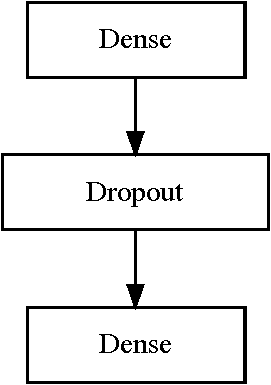
\includegraphics[width=0.2\textwidth]{graphics/text-classification/model.pdf}
% \end{wrapfigure}

    \todo[inline]{- Input layer bei diesen Grafiken ergänzen
    
    - Breite der Layer in der Grafik ergänzen}
\end{figure} 

Während dem Experiment wurde die optimale Grösse des Wörterbuchs durch Ausprobieren ermittelt. Es wurde dabei festgestellt, dass das Modell mit einem grösseren Wörterbuch von 5000 Wörtern die besten Ergebnisse liefert. Je grösser das Wörterbuch, desto schneller hat das Modell begonnen Auswendig zu lernen (Overfitting). Um diesem Effekt entgegenzuwirken wurde ein grosser Dropout von 0.92 gewählt. Auch dieser Wert wurde empirisch ermittelt.

Bei dem gewählten Modell, mit einem Vokabular von 5000 Wörtern und einem Dropout von 0.92, erreicht das loss auf den Testdaten nach 23 Epochen Training den Wendepunkt (vgl. Abbildung \ref{text-class-results:val_loss}). Dabei wird eine Treffergenauigkeit von 98.4\% erzielt (vgl. Abbildung \ref{text-class-results:val_acc}). 

\begin{figure}[h!] 
  \captionsetup{width=.8\linewidth}
  \caption[Statistiken aus dem Training der Text-basierten Klassifizierung von Rechnungen]{Statistiken aus dem Training der Text-basierten Klassifizierung von Rechnungen.}
  \label{text-class-results}
  \begin{subfigure}[b]{0.5\linewidth}
    \centering
    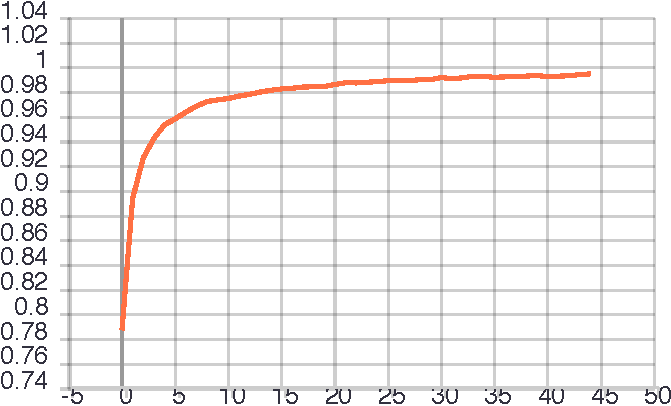
\includegraphics[width=0.75\linewidth]{graphics/text-classification/acc.pdf} 
    \caption{Treffergenauigkeit} 
    \label{text-class-results:val} 
    \vspace{2ex}
  \end{subfigure}%% 
  \begin{subfigure}[b]{0.5\linewidth}
    \centering
    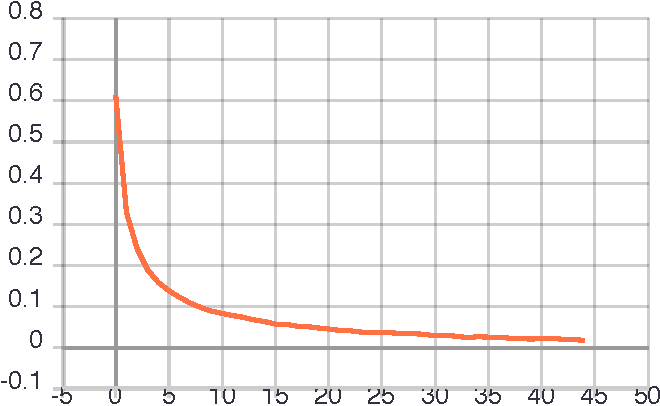
\includegraphics[width=0.75\linewidth]{graphics/text-classification/loss.pdf} 
    \caption{loss} 
    \label{text-class-results:loss} 
    \vspace{2ex}
  \end{subfigure} 
  \begin{subfigure}[b]{0.5\linewidth}
    \centering
    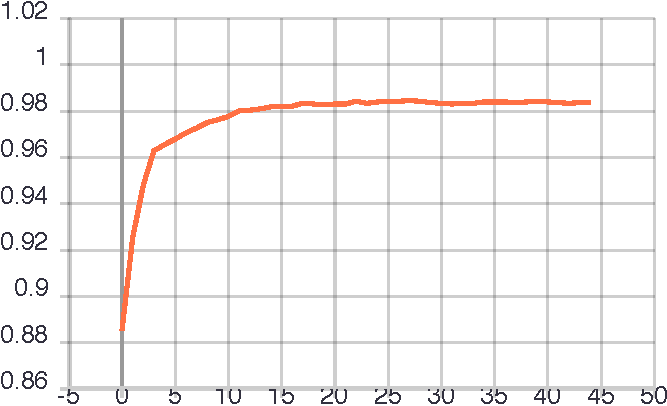
\includegraphics[width=0.75\linewidth]{graphics/text-classification/val_acc.pdf} 
    \caption{Treffergenauigkeit bei den Testdaten} 
    \label{text-class-results:val_acc} 
  \end{subfigure}%%
  \begin{subfigure}[b]{0.5\linewidth}
    \centering
    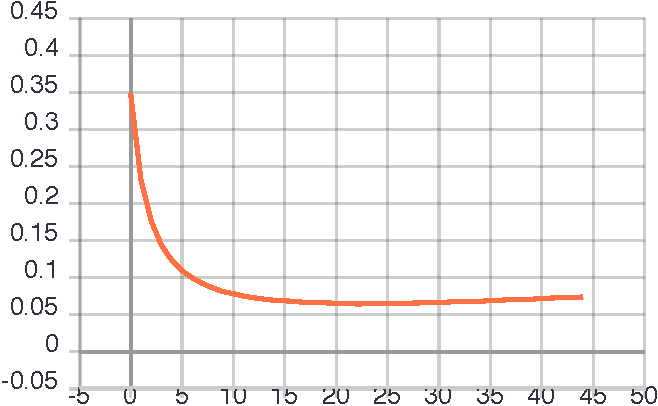
\includegraphics[width=0.75\linewidth]{graphics/text-classification/val_loss.pdf} 
    \caption{loss bei den Testdaten} 
    \label{text-class-results:val_loss} 
  \end{subfigure}
  \centering
\end{figure}

Die falsche Klassifizierung einer Rechnung ist vor allem dann problematisch, wenn diese einer Klasse zugewiesen wird, welche automatisch Verarbeitet wird. Die Confusion Matrix in Abbildung \ref{text-classification-cm} zeigt, dass das Text-basierte Modell 6 aus 3367 Rechnungen des Testsets fälschlicherweise als Fitness Rechnungen und 5 Rechnungen fälschlicherweise als Rechnungen für einen Sportverein klassifiziert hat. Dies ergibt eine Genauigkeit (Precision) von 97.86\% (Fitness), 100\% (Optiker) respektive 96.50\% (Sportverein).

\todo[inline]{Precision und Recall anhand der Confusion Matrix besprechen. Error analysis, wie dies im Buch Machine Learning Yearning beschrieben ist beschreiben. Daraus die Fehler/das Potential, welche unten folgend, ableiten und ergänzen.}

\begin{figure}[h!] 
%\begin{wrapfigure}{r}{0.5\textwidth} 
    \caption[Confusion Matrix des Text-basierten Modells zur Klassifizierung von Rechnungen]{Confusion Matrix nach 23 Epochen Training des Text-basierten Modells zur Klassifizierung von Rechnungen. Das Modell klassifiziert sechs Rechnungen fälschlicherweise als Fitness Rechnung und fünf Rechnungen fälschlicherweise als Rechnungen für einen Sportverein.}
    \label{text-classification-cm}
    \centering
    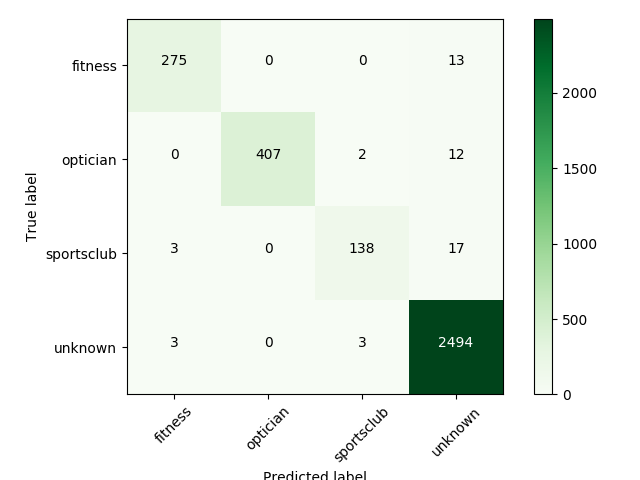
\includegraphics[width=0.8\textwidth]{graphics/text-classification/cm_22.png}
%\end{wrapfigure}
\end{figure}

Die Insgesamt 53 falsch klassifizierten Rechnungen aus dem Testdatensatz sowie die während dem Training falsch klassifizierten Rechnungen wurden einer Fehleranalyse unterzogen. \textcite{MLYearning} suggerieren für die Verbesserung eines Modells dort anzusetzen, wo am meisten Falschklassifikationen vorliegen. Dabei wird argumentiert, dass dort das Potential, die Treffergenauigkeit zu erhöhen, am höchsten ist. In unserem Fall ist die Treffergenauigkeit aber eher nebensächlich. Die 42 fälschlicherweise als Übrigen klassifizierten Rechnungen haben keinen grossen negativen Einfluss auf den Geschfätsprozess. Aus diesem Grund fokussiert sich die Analyse auf die fälschlicherweise als eine der automatisierbaren Klassen klassifizierten Rechnungen. Während dieser Analyse wurden folgende Probleme identifiziert:

\textbf{Ungenauigkeiten der Optical Chracter Recognition}

Ein Problem, welches sofort ins Auge sticht, sind die Ergebnisse des Optical Character Recognition Systems. Diese sind teilweise sehr dürftig. Durch die mässige Qualität fotografierter Rechnungen können gewisse Wörter nur schlecht oder garnicht erkannt werden. 

Durch diese Ungenauigkeiten während dem OCR Prozess entstehen viele Wörter mit Schreibfehlern. Das Wörterbuch erkennt aber nur Wörter, welche mit den gelernten Wörtern identisch sind. Wurde während dem Training des Wörterbuchs ein Wort nie in einer gewissen falschen Schreibweise angetroffen, so ist dieses Wort für das Klassifizierungsmodell nutzlos.

Eine Problematik für das Optical Character Recognition System ist eine schlechte Ausleuchtung des Fotos einer Rechnung. In diesem Fall erkennt das OCR System nur sehr wenig bis überhaupt kein Text. Dadurch kann die Rechnung nicht klassifiziert werden.

Eine weitere Problematik ist ein körniges Bild. In diesem Fall erkennt das OCR System diakritische Zeichen wie ein é, wo keine sind. Dadurch kann ein Wort nicht im Wörterbuch gefunden werden und es trägt somit nicht zur Klassifizierung bei.

\textbf{Überrepräsentation einzelner Wörter in gewissen Klassen}

Die Fielmann AG ist wohl einer der bekanntesten Optiker in der Schweiz. Sehen wir eine Rechnung und lesen Fielmann, denken wir sofort an eine Optiker Rechnung. Genau so scheint auch unser Modell zu denken, denn eine Rechnung von Fielmann wird stets als Optiker Rechnung klassifiziert. Dies stellt nun aber ein Problem dar, denn Fielmann verkauft nicht nur Seh- sondern auch Hörhilfen.

Diese Problematik erinnert an das Problem der überrepräsentierten Klassen. Auf Stufe der Klassen trägt die Gewichtung der loss Function der Überrepräsentation einzelner Klassen Rechnung. Auf der Stufe des Vokabulars wird dies bis anhin nicht gemacht.

\todo[inline]{Literatur zu diesem Problem suchen.

Potentielle Lösungen:

- Blacklisting des Begriffs "fielmann". Analog andere grosse Gewichte im neuronalen Netzwerk suchen und diese Begriffe blacklisten

- Undersampling von fielmann Optiker Rechnungen}

\textbf{Nicht eindeutige Wahrscheinlichkeiten bei der Klassifizierung}

Die verwendete Methode der Klassifizierung verwendet vier Wahrscheinlichkeiten, mit welcher eine Rechnung einer bestimmten Klasse angehört. In Summe ergeben diese Wahrscheinlichkeiten immer 1. Die Klasse, bei welcher die Wahrscheinlichkeit am höchsten liegt, gewinnt. Es kann nun vorkommen, dass die Wahrscheinlichkeiten annähernd gleichmässig verteilt sind und eine Rechnung mit einer Klassen-Wahrscheinlichkeit von nur 25.1\% klassifiziert wird.

\textbf{Klassifizierung aufgrund irrelevanter Wörter}

Bei der Betrachtung einiger Rechnungen wurde festgestellt, dass diese hauptsächlich aus einem Einzahlungsschein bestehen. Dies kam besonders oft bei Sportvereinen vor und somit assoziert das Modell nun Wörter, welche auf dem Orangen Einzahlungsschein vorhanden sind, mit einer Rechnung eines Sportvereins.

\hspace{10cm}

\todo[inline]{Verbesserungsvorschläge direkt bei der Fehleranalyse mit einfliessen lassen? Eigenes Kapitel?}

\hspace{10cm}

\textbf{OCR Fehler}

Um die Resultate dieses Zwischenschritts zu verbesseren, sieht der Autor folgende Optionen.

\begin{itemize}
    \item Es könnte versucht werden, dass LSTM Modell, welches dem Tesseract OCR System zugrunde liegt, auf die Rechnungen zu trainieren. Das OCR System kann durch Training mit Schriftzügen und Buchstaben, auf welche das System bisher nicht Trainiert wurde, einiges an Treffergenauigkeit gewinnen. Das System sollte aus diesem Grund auf die gängigsten Schriften der Rechnungen trainiert werden\~{TesseractTraining}.
    \item Aktuell wurde das OCR System mit den Sprachen Deutsch, Englisch, Französisch und Italienisch instruiert. Nach dem ersten Lauf mit diesen vier Sprachen könnte versucht werden, mit einem KI-Modell die Sprache zu erkennen. Anschliessen könnte das OCR System mit nur dieser Sprache erneut verwendet werden. Somit könnten beispielsweise falsche diakritische Zeichen durch eine Körnung des Bildes vermindert werden. Auch erlaubt dieses Vorgehen dem OCR System die verbesserte Erkennung durch dem System bekannte Wörter.
    \item Die Ergebnisse aus dem OCR Schritt könnten durch ein Rechtschreibe- und Grammatikkorrektur-Modell verbessert werden. \todo{Referenz auf Einleitungskapitel}
    \item Image preprocessingwith OpenCV (rectification, ...)
\end{itemize}

\textbf{Verbessertes WordEmbedding}

Anstelle des aktuell verwendeten, einfachen Word Tokenizer könnte ein komplexeres WordEmbedding\todo{Referenz auf Einleitungskapitel} angewendet werden. Jüngste Forschungen zeigen, dass auch in diesem Bereich dank Transfer Learning gute Ergebnisse erzielt werden können. Beispielsweise wurde im Oktober 2018 mit BERT\footnote{Bidirectional Encoder Representations from Transformers, kurz BERT, ist ein Modell zur repräsentation von natürlicher Sprache. Das Modell des Google Reasearch Team bricht viele bisherige Rekorde bei Natural Language Processing Wettbewerben~\autocite{Devlin2018}} ein sehr erfolgreiches Modell im Bereich des Natural Language Processing publiziert, welches als Grundlage für das Transfer Learning dienen kann~\autocite{Devlin2018}.

\textbf{Probability}

Die Probability der Klassen mit einfliessen lassen. Dem Modell erlauben, zu sagen, es wisse es nicht

\todo[inline]{
Klassifizierung von Rechnungen

Evtl. verschiedene Ansätze

- OCR -> (SpellCorrection ->) WordEmbedding -> classification

- Pixel -> classification

- OCR -> (SpellCorrection ->) InformationExtraction -> classification

Bewertung der Ergebnisse
}

\todo[inline]{Dropout und dilating beschreiben}